% ----------------------------------------------------------------------------------------------------- %
% Capítulo 3 - FUNDAMENTAÇÃO TEÓRICA
% ----------------------------------------------------------------------------------------------------- %
\chapter{Fundamentação Teórica}
\label{cap:teoria}

\noindent Ao longo desse capítulo estão expostos conceitos básicos que são de grande importância para o entendimento deste trabalho e dentre eles serão destacados: definição de matriz, principais matrizes utilizadas no estudo da Álgebra Linear, sistemas de equações lineares, conteúdo este que fará parte da plataforma de ensino e aprendizagem AlfaGebra, espaço vetorial que também irá compor o AlfaGebra. Também uma abordagem sobre engenharia de \textit{software} a fim de explanar como consiste o desenvolvimento de um sistema, e para um desenvolvimento mais organizado a utilização da metodologia ágil, em especial o \textit{framework Scrum} será aplicada no desenvolvimento do \textit{software} AlfaGebra. E para a implementação da plataforma de ensino e aprendizagem AlfaGebra será aplicado a computação simbólica como recursos para o tratamento das expressões que será fornecidas pelos os usuários e outros aplicações. Será discutido também uma abordagem do \textit{software} Matlab como ferramenta de aprendizagem e resolução de problemas e por fim, uma abordagem sobre avaliação do ensino e aprendizagem.

\section{Matrizes}
\noindent Um das ferramentas mais poderosas consideradas na matemática são as matrizes, pois as mesmas tem aplicações em diversas áreas, tais como em codificação e decodificação de mensagens, computação gráfica, engenharias, etc. Desse modo, faz-se necessário a compreensão de algumas propriedades e nomenclaturas em relação as mesmas.

\subsection{Definição de matriz}
\noindent Matrizes são objetos matemáticos estruturados em tabelas disposta em $m$ linhas e $n$ colunas. A definição de Steinbruch \cite{1987:Steinbruch} é similar a citada, onde uma matriz é uma tabela $m x n$ de elementos, e que estes podem ser números, polinômios, funções, etc., que estão dispostos em $m$ linhas e $n$ colunas, representada por  $A{}_{mxn}$.\\

\begin{center}
    $A = 
    \begin{bmatrix}
        a_{11} & a_{12} & a_{13} & \ldots & a_{1n}\\ 
        a_{21} & a_{22} & a_{23} & \ldots & a_{2n}\\ 
        a_{31} & a_{32} & a_{33} & \ldots & a_{3n}\\ 
        \vdots & \vdots & \vdots & \ldots & \\ 
        a_{m1} & a_{m2} & a_{m3} & \ldots & a_{mn}
    \end{bmatrix}_{mxn}$
\end{center}

%
\subsection{Tipos de matrizes}
\noindent Para Boldrini \cite{1980:Boldrini}, no processo de utilização de matrizes, percebe-se que existem algumas que são diferentes, seja pela quantitativo de linhas ou colunas, bem como também pela natureza de seus elementos, a qual apresentam propriedades que se diferenciam de uma matriz qualquer. A seguir, serão expostas as principais categorias de matrizes, para isso, considerando uma matriz com $m$ linhas e $n$ colunas representa por $A{}_{mxn}$.

\subsubsection{Matriz Quadrada}
\noindent Quando o número de linhas $m$ é igual ao número de coluna $n$ $(m = n)$.

\textit{Exemplo:}
\begin{center}
    $A = 
    \begin{bmatrix}
        a_{11} & a_{12} & a_{13} \\ 
        a_{21} & a_{22} & a_{23} \\ 
        a_{31} & a_{32} & a_{33} 
    \end{bmatrix}_{mxn}$
\end{center}

Observando a matriz $A$, percebe-se que o número de linhas e colunas são iguais, sendo $A{}_{3x3}$. Nesse tipo de matriz, em que a ordem é $n$ por $n$, costuma dizer que $A$ é uma matriz de ordem $n$.

\subsubsection{Matriz Linha}
\noindent A matriz que apresenta somente uma linha, ou seja, matriz de ordem $1$ por $n$.

\textit{Exemplo:}
\begin{center}
    $A = 
    \begin{bmatrix}
        a_{1} & a_{2} & a_{3} & \ldots & a_{n}
    \end{bmatrix}_{1 x n}$
\end{center}

\subsubsection{Matriz Coluna}
\noindent A matriz que apresenta somente uma coluna, ou seja, matriz de ordem $n$ por $1$.

\textit{Exemplo:}
\begin{center}
    $A = 
    \begin{bmatrix}
        a_{1} \\ 
        a_{2} \\
        a_{3} \\
        \vdots \\
        a_{n} 
    \end{bmatrix}_{n x 1}$
\end{center}

\subsubsection{Matriz Nula}
\noindent A matriz cujos elementos $A{}_{ij}$ são todos nulos.

\textit{Exemplo:}
\begin{center}
    $A = 
    \begin{bmatrix}
        0 & 0 & 0\\ 
        0 & 0 & 0 
    \end{bmatrix}$
\end{center}

\subsubsection{Matriz Diagonal}
\noindent É uma matriz quadrada $A = \begin{bmatrix} a_{}_{ij} \end{bmatrix}$ em que os elementos que não pertencem a diagonal principal são todos nulos, denotada por $A{}_{ij} = 0$, para $i \neq j$.

\textit{Exemplo:}
\begin{center}
    $A = 
    \begin{bmatrix}
        a_{11} & 0 & 0 \\ 
        0 & a_{22} & 0 \\ 
        0 & 0 & a_{33}  
    \end{bmatrix}$
\end{center}

\subsubsection{Matriz Identidade}
\noindent A matriz escalar de qualquer ordem, que tem todos os elementos da diagonal principal $A{}_{ij} = 1$, para todo $i \neq j$. Representada com $I{}_{n}$, ou simplesmente por $I$ é chamada de matriz identidade.

\textit{Exemplo:}
\begin{center}
    $I_{3} = 
    \begin{bmatrix}
        1 & 0 & 0 \\ 
        0 & 1 & 0 \\ 
        0 & 0 & 1  
    \end{bmatrix}$
\end{center}

\subsection{Operações com matrizes}
\noindent Para uma melhor utilização das matrizes é necessário um entendimento sobre as operações aritméticas aplicadas nelas. Assim, a seguir serão demonstradas as três operações que são aplicadas nelas.

\subsubsection{Multiplicação por um escalar}
\noindent De acordo coma definição de Leon \cite{1998:Leon}, se $A$ é uma matriz e $\alpha$ é um escalar, assim $\alpha A$ será a matriz gerada a partir da multiplicação de cada elemento de $A$ por $\alpha$.

\textit{Exemplo:}
\begin{center}
    $5 \cdot
    \begin{bmatrix}
        1 & 3 & 6 \\ 
        -4 & 2 & 0 \\ 
        5 & 7 & -1  
    \end{bmatrix}
    =
    \begin{bmatrix}
        5 \cdot 1 & 5 \cdot 3 & 5 \cdot 6 \\ 
        5 \cdot (-4) & 5 \cdot 2 & 5 \cdot 0 \\ 
        5 \cdot 5 & 5 \cdot 7 & 5 \cdot (-1)  
    \end{bmatrix}
    =
    \begin{bmatrix}
        5 & 15 & 30 \\ 
        -20 & 10 & 0 \\ 
        25 & 35 & -5
    \end{bmatrix}$
\end{center}

Em relação as propriedades da multiplicação de uma matriz por um escalar, para quaisquer matrizes $A$ e $B$ de mesma ordem e os escalares $\alpha$ e $\lambda$ $\in \mathbb{R}$, a multiplicação por o escalar satisfaz as presentes propriedades:
\begin{enumerate}
    \item[i)] $(\alpha \lambda) A = \alpha(\lambda A)$
    \item[ii)] $(\alpha + \lambda) A = \alpha A + \lambda A$
    \item[iii)] $\alpha(A + B) = \alpha A + \alpha B)$
    \item[iv)] $1 A = A$
\end{enumerate}
 
\subsubsection{Soma de matrizes}
\noindent Dadas duas matrizes  $A = \begin{bmatrix} a_{}_{ij} \end{bmatrix}$ e  $B = \begin{bmatrix} b_{}_{ij} \end{bmatrix}$ de ordem $(i, j)$. Assim, a soma $A + B$ é uma matriz  $C = \begin{bmatrix} c_{}_{ij} \end{bmatrix}$.

\textit{Exemplo:}
\begin{center}
    $A =
    \begin{bmatrix}
        a{}_{11} & a{}_{12} & a{}_{13} \\ 
        a{}_{21} & a{}_{22} & a{}_{23} 
    \end{bmatrix}
    $
    e
    $B =
    \begin{bmatrix}
        b{}_{11} & b{}_{12} & b{}_{13} \\ 
        b{}_{21} & b{}_{22} & b{}_{23}
    \end{bmatrix}$
\end{center}

então:

\begin{center}
    $
    \begin{bmatrix}
        a{}_{11} & a{}_{12} & a{}_{13} \\ 
        a{}_{21} & a{}_{22} & a{}_{23} 
    \end{bmatrix}
    +
    \begin{bmatrix}
        b{}_{11} & b{}_{12} & b{}_{13} \\ 
        b{}_{21} & b{}_{22} & b{}_{23}
    \end{bmatrix}
    =
    \begin{bmatrix}
        a{}_{11} + b{}_{11} & a{}_{12} + b{}_{12} & a{}_{13} + b{}_{13} \\ 
        a{}_{21} + b{}_{21} & a{}_{22} + b{}_{12} & a{}_{23} + b{}_{13}
    \end{bmatrix}$
\end{center}
Em relação às propriedades da adição de matrizes, para quaisquer matrizes $A, B$ e $C$ de mesma ordem $i \times j$, existem as seguintes propriedades que a satisfazem:

\begin{enumerate}
    \item[i)] $A + (B + C) = (A + B) + C$
    \item[ii)] $A + 0 = 0 + A = A$
    \item[iii)] $-A + A = A - A = 0$
    \item[iv)] $A + B = B + A$
\end{enumerate}

\subsubsection{Multiplicação de matrizes}
\noindent Uma das operações mais importantes entre matrizes é a multiplicação. De acordo com Leon \cite{1998:Leon}, a motivação da definição de multiplicação entre matrizes vem de sua aplicação em sistemas lineares.

Boldrini \cite{1980:Boldrini} define: sejam $A = \begin{bmatrix} a_{}_{ij} \end{bmatrix}_{m \times n}$ e $B = \begin{bmatrix} b_{}_{rs}\end{bmatrix}_{n \times p}$. Assim defini-se $C = \begin{bmatrix} c_{}_{uv} \end{bmatrix}_{m \times p}$, onde

\begin{center}
    $c_{uv} = \sum_{k = 1}^{n} a_{uk}b_{kv} = a_{u1}b_{1v} + ... + a_{un}b_{nv}$
\end{center}

Desse modo, para formar o elemento $C_{ij}$ do produto, pega-se a \textit{i-ésima} linha de $A$ e a \textit{j-ésima} coluna de $B$, e assim multiplicam-se os elementos correspondentes dois a dois e soma-se os números resultantes. Contudo, para efetuar o produto entre duas matrizes $A_{m \times n}$ e $B_{l \times p}$, só é possível se o número de colunas da primeira for igual ao número de linhas da segunda, isto é, $n = 1$. Além disso, o resultado da matriz $C = A\cdot B$ será de ordem $m \times p$.

\textit{Exemplo:}
\begin{center}
    $A = 
    \begin{bmatrix}
        1 & 2 & 3 \\ 
        -2 & 1 & 6 
    \end{bmatrix}$
    e $B = 
    \begin{bmatrix}
        3 & -2 \\ 
        2 & 4 \\
        1 & -3 
    \end{bmatrix}$
\end{center}

então:

\begin{center}
    $AB =
    \begin{bmatrix}
        1 \cdot 3 + 2 \cdot 2 + 3 \cdot 1 & 1 \cdot (-2) + 2 \cdot 4 + 3 \cdot (-3) \\ 
        (-2) \cdot 3 + 1 \cdot 2 + 6 \cdot 1 & (-2) \cdot (-2) + 1 \cdot 4 + 6 \cdot (-3)
    \end{bmatrix}
    =
    \begin{bmatrix}
        10 & -3 \\ 
        2 & -10 
    \end{bmatrix}$
\end{center}

\section{Sistemas de Equações Lineares}
\noindent Na matemática, provavelmente um dos problemas considerados mais importantes é a resolução de sistemas de equações lineares. Leon \cite{1998:Leon} destaca a importância desse conteúdo na Álgebra Linear, visto que muitos dos problemas matemáticos que são encontrados em aplicações científicas e industriais abordam em alguma etapa do processo a resolução de um sistema linear. Usando os métodos matemáticos modernos, em muitos dos casos é possível minimizar o problema a um único sistema de equações lineares. E as aplicações e utilização de sistemas de equações lineares está presente em várias áreas como administração, sociologia, economia, ecologia, demografia, engenharia, física, genética, entre outras.

\subsection{Equação Linear}
\noindent Por definição uma equação linear é uma equação da forma: 
\begin{center}
    $a_{1}x_{1} + a_{2}x_{2} + a_{3}x_{} + ... + a_{n}x_{n} = b$   
\end{center}
onde $a_{1}, a_{2}, ..., a_{n}$ são os coeficientes, $x_{1}, x_{2}, ..., x_{n}$ são incógnitas e b é o termo independente.

\subsection{Sistemas de equações lineares}
\noindent Um sistema de equações lineares refere-se a um conjunto de equações do tipo:\\

$\left\{\begin{matrix}
    a_{11}x_{1} + a_{12}x_{2} + a_{13}x_{3} + \ldots + a_{1n}x_{n} = b_{1}\\ 
    a_{21}x_{1} + a_{22}x_{2} + a_{23}x_{3} + \ldots + a_{2n}x_{n} = b_{2}\\ 
    a_{31}x_{1} + a_{32}x_{2} + a_{33}x_{3} + \ldots + a_{3n}x_{n} = b_{3}\\ 
    \ldots\\ 
    a_{m1}x_{1} + a_{m2}x_{2} + a_{m3}x_{3} + \ldots + a_{mn}x_{n} = b_{m}\\ 
\end{matrix}\right$

\subsection{Operações Elementares}
\noindent As operações elementares sobre as linhas de uma matriz são um total de três:
\begin{itemize}
    \item Permutação de duas linhas $(L_{i} \rightarrow L_{j})$:\\
    \textit{Exemplo:}\\
    $L_{2} \rightarrow L_{3}$
    $\begin{center}
        \begin{bmatrix}
         1 & 1\\ 
         5 & 0\\ 
         -3 & 4
        \end{bmatrix}
        \rightarrow 
        \begin{bmatrix}
         1 & 1\\ 
         -3 & 4\\ 
         5 & 0
        \end{bmatrix}\\
    \end{center}$\\
\end{itemize}

\begin{itemize}
    \item Multiplicação de uma linha por um escalar $k$, não nulo. $(L_{i} \rightarrow k\cdot L_{i})$:\\
    \textit{Exemplo:}\\
    $L_{2} \rightarrow 2 \cdot L_{2}$
    $\begin{center}
        \begin{bmatrix}
         1 & 1\\ 
         5 & 0\\ 
         -3 & 4
        \end{bmatrix}
        \rightarrow 
        \begin{bmatrix}
         1 & 1\\ 
         10 & 0\\ 
         -3 & 4
        \end{bmatrix}\\
    \end{center}$\\
\end{itemize}

\begin{itemize}
    \item Substituição de uma linha por sua soma com outra equação previamente multiplicada por um escalar $k$ não nulo $(L_{i} \rightarrow L_{i} + k \cdot L_{j})$:\\
    \textit{Exemplo:}\\
    $L_{2} \rightarrow L_{2} + 2 \cdot L_{1}$
    $\begin{center}
        \begin{bmatrix}
         1 & 1\\ 
         5 & 0\\ 
         -3 & 4
        \end{bmatrix}
        \rightarrow 
        \begin{bmatrix}
         1 & 1\\ 
         7 & 2\\ 
         -3 & 4
        \end{bmatrix}$\\
    \end{center}
\end{itemize}

\subsection{Forma Escada}
\noindent Por definição dada por Boldrini \cite{1980:Boldrini}, uma matriz de dimensões $m \times n$ é considerada linha reduzida à forma escada se atender aos presentes requisitos abaixo:

\begin{enumerate}
    \item O primeiro elemento de cada linha diferente de zero é igual a 1.
    \item Cada coluna que apresenta o primeiro elemento diferente de zero de alguma linha tem todos os demais elementos iguais a zero.
    \item Se existirem linhas com todos os elementos iguais a zero, elas ficam abaixo de todas as linhas não-nulas.
    \item O número de zeros que precede o primeiro elemento não nulo, aumenta a cada linha.
\end{enumerate}

\subsubsection{Definição:}
\noindent Dada uma matriz $A_{m \times n}$, seja $B_{m \times n}$ a matriz linha reduzida à forma escada de $A$. O posto de $A$, denotado por $P$ é a quantidade de linhas não nulas de $B$ e a nulidade de $A$ é o número $n-p$.

\subsection{Soluções de um sistema de equações lineares}
\noindent Dentro da resolução de sistemas de equações lineares podem ocorrer diversas situações na resolução. Considerando um sistema de uma equação e um incógnita $ax = b$, existirão três possibilidades:
\begin{enumerate}
    \item O sistema possui uma única solução. O sistema nesse caso é dito compatível e determinado ou sistema possível e determinado.
    \item Sistema possui infinitas soluções. O sistema é dito compatível e indeterminado ou sistema possível e indeterminados.
    \item Sistema não possui solução. O sistema é dito incompatível ou impossível. 
\end{enumerate}

\section{Espaço Vetorial}
\noindent Leon \cite{1998:Leon} explana que ``as operações de soma e multiplicação por um escalar são usadas em diversos contextos em matemática. Independentemente do contexto, no entanto, essas operações obedecem, em geral, ao mesmo conjunto de regras aritméticas". E diante de tal, aplicações de sistemas matemáticos que abordam as operações de soma e multiplicação por um escalar apresentam aplicações em várias áreas da matemática e esses sistemas matemáticos desse modelo são chamados de espaços vetoriais. 

Abramo \cite{2016:Abramo} destaca que espaço vetorial está presente em zonas importantes da análise matemática e da geometria diferencial. A utilização de espaços vetoriais está presente em diversas aplicações e áreas, dentre algumas delas, a computação gráfica com sua utilização no espaço espectral de cores, no sistema RGB (\textit{Red, Green e Blue}), em aplicações na física moderna, entre outras.

\subsection{Espaços Vetoriais}
\subsubsection{Definição}
\noindent Boldrini \cite{1980:Boldrini} defini um espaço vetorial real como um conjunto $V$, não vazio, com as seguintes operações: soma, $V\times V\overset{+}{\rightarrow}V$ e a multiplicação por escalar, $\mathbb{R}\times V\overset{\cdot}{\rightarrow}V$ assim, para quaisquer $u, v, w$ e $a, b \in \mathbb{R}$, as propriedades são satisfeitas.

\subsubsection{Operação soma}
\begin{enumerate}
    \item $(u + v) + w = u + ( v + w)$
    \item $u + v = v + u$
    \item Existe $0 \in v$ tal que $0 + v = v$ (0 é chamado vetor nulo)
    \item Existe $- u \in v$ tal que $u + (-u) = 0$
\end{enumerate}
\subsubsection{Operação multiplicação}
\begin{enumerate}
    \item $a(u + v) = au + av$
    \item $(a + b)v = av + bv$
    \item $(ab)v = a(bv)$
    \item $1u = u$
\end{enumerate}

\subsection{Subespaços Vetoriais}
\noindent Em alguns casos é necessário descobrir dentro de um espaço vetorial $V$, subconjuntos $W$ que sejam eles próprios espaços vetoriais menores. Estes conjuntos são chamados de subespaços de $V$. Por exemplo, considerando $V = \mathbb{R}^{2}$ o plano onde $W$ é uma reta deste plano, que passa pela origem.

\begin{figure}[!hb]
  \centering 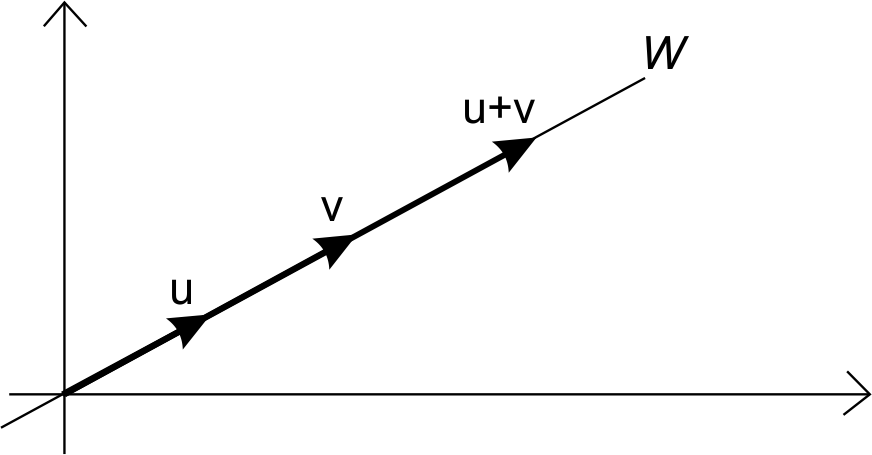
\includegraphics[dimensões]{Figuras/subespacos.png}
  \caption{Subespaço.}
  \label{chave_para_refencia_cruzada}
\end{figure}

\subsubsection{Definição:}
\noindent Dado um espaço vetorial de $V$, um subconjunto $W$, não vazio, será um espaço vetorial de $V$ se atender as duas condições:

\begin{enumerate}
    \item $\forall u, v \in W \rightarrow u + v \in W$
    \item $\forall \alpha \in \mathbb{R}$ e $u \in W \rightarrow \alpha u \in W$
\end{enumerate}

\textit{Exemplo:}\\
Nesse exemplo verifica se o conjunto $W = \left \{ (x, 2x) ; x \in \mathbb{R} \right \} \subset \mathbb{R}^2$ é um subespaço vetorial.

Inicialmente deve-se verificar se o vetor nulo está incluso no subespaço, assim:
\begin{center}
    $(0, 2\cdot0) = (0,0) \in W$    
\end{center}
Como a verificação é válida, o vetor nulo encontra-se dentro do subespaço, agora analisando as condições da definição:

\subsubsection{Condição 1}
\noindent Sejam $u = (x_{1}, 2x_{1}), v = (x_{2}, 2x_{2}) \in W$. Verificando se $u + v \in W$:
\begin{center}
    $u + v = (x_{1}, 2x_{1}) + (x_{2}, 2x_{2})$\\
    $u + v = (x_{1} + x_{2}, 2x_{1}) + 2x_{2})$\\
    $u + v = (x_{1} + x_{2}, 2(x_{1} + x_{2})) \in W$\\
\end{center}
Observando o resultado obtido percebe-se que a ordenada é o dobro da abscissa.

\subsubsection{Condição 2}
\noindent Sejam $\alpha \in \mathbb{R}$ e $u = (x_{1}, 2x_{1}) \in W$. Verificando se $\alpha u \in W$:
\begin{center}
    $\alpha u = \alpha(x_{1}, 2x_{1})$\\
    $\alpha u = (\alpha x_{1}, \alpha 2x_{1})$\\
    $\alpha u = (\alpha x_{1}, 2(\alpha x_{1})) \in W$\\
\end{center}
Como as duas condições são satisfeitas, então o conjunto é um subespaço vetorial.


\section{Computação simbólica}
\noindent A computação apresenta limitação no que tange a capacidade de armazenamento de dados, em virtude disso, nas operações de cálculos, os arredondamentos são aplicados e acabam afetando a precisão da resposta esperada. Mas, a computação simbólica apresenta uma diferencial neste quesito, pois na computação simbólica os dados são armazenados como frações e manipulados algebricamente, o que ocasiona a precisão da resposta total. Destarte, ela é bastante utilizada na matemática para manipular formas simbólicas de expressões matemáticas e para realizar cálculos numéricos que são utilizados em \textit{softwares} numéricos.

Assim, a computação simbólica é um ramo da Ciência da Computação e Matemática que estuda as operações simbólicas que são tratadas por um computador, ou seja, o desenvolvimento de algoritmos para manipulação de expressões matemáticas e outros objetos matemáticos \cite{2005:Leandro}.

Em sistemas de computação simbólica, Bortolossi \cite{2012:Humberto} descreve que são
\begin{quote}
    \textit{softwares} matemáticos que permitem lidar com símbolos e obter respostas exatas para muitos problemas matemáticos, como a fatoração de números inteiros e polinômios, operações com matrizes, resolução de sistemas de equações lineares e não lineares, operações com números complexos, simplificações de expressões, cálculo de limites, derivadas e integrais, resolução de equações diferenciais, etc. (p. 1).
\end{quote}

Já Campos \cite{2015:Lidio}, explana que é
\begin{quote}
    um interessante recurso de programação de alto nível, que integra os paradigmas de programação procedural, programação funcional e programação baseada em regras, que permite aos programadores especialistas produzirem aplicações que sistematicamente trabalham o desenvolvimento de cálculo analítico avançado (p. 4).  
\end{quote}

Muitas aplicações na matemática, ciências e engenharias requerem operações simbólicas na resolução de operações, a partir disso, nas últimas décadas, no que tange o desenvolvimento de \textit{software} para matemática, foram desenvolvidos vários sistemas entre alguns deles o Mathematica, Maple, Matlab, Mupad, entre outros que permitem a manipulação simbólica de expressões matemáticas, e assim possibilitando resultados exatos e dentre estes \textit{softwares} os que mais recebem destaque são o Maple e Mathematica, devido a sua capacidade de resolução \cite{2007:Valesca}. É importante salientar que todos esses sistemas trabalham com os conteúdos da Álgebra Linear e por conseguinte, utilizam a computação simbólica para resolução dos problemas.

\section{\textit{Software} matemático com abordagem em Álgebra Linear}
\noindent Com o avanço das tecnologias muitos \textit{softwares} foram desenvolvidos com o propósito de auxiliar no aprendizado e na resoluções de problemas matemáticos, dentre alguns deles, o  Matlab\footnote[2]{Matlab \url{https://www.mathworks.com/products/matlab.html}} que é ambiente computacional para trabalho com expressões algébricas e simbólicas, o Maple\footnote[3]{Maple \url{https://www.maplesoft.com/}} também é outro \textit{software} computacional específico para resoluções de problemas matemáticos e constitui um ambiente computacional para o trabalho de expressões algébricas e simbólicas, outro é Mathematica\footnote[4]{Mathematica \url{https://www.wolfram.com/mathematica/}} que é um \textit{software} que trabalha com álgebra computacional e utiliza expressões algébricas e simbólicas para resolução, e foi desenvolvido pela Wolfram Research, entre alguns outros. Em virtude do Matlab ser um \textit{software} conhecido mundialmente e por ser uma ferramenta poderosa o mesmo será abordado com aspectos ligados à abordagem da Álgebra Linear.

\subsection{Matlab}
\noindent Matlab é um \textit{software} poderoso, ``conhecido mundialmente como uma excelente ferramenta para soluções de problemas matemáticos, científicos e tecnológicos, que possui comandos muito próximos da forma como são escritas as expressões matemáticas"  (\cite{2005:Marcello}, 2005, p. 2). Sua aplicação é usada para resoluções de problemas em diversas áreas, tais como: processamento de imagens, animação, aprendizagem profunda, visão computacional, robótica, etc. \cite{2004:Wu}. Trata-se de um \textit{software} interativo de alta performance voltado para o cálculo numérico, desenvolvido no final dos anos de 1970 pelo o presidente do departamento de ciência da computação da Universidade do Novo México, Cleve Moler\footnote[1]{Cleve Moler é PhD pela Universidade de Stanford em Matemática, presidente e cofundador da MathWorks. Moler é matemático e cientista da computação, trabalha com Álgebra Linear numérica e desenvolveu \textit{software} Matlab \cite{2016:Raquel}.} \cite{2016:Raquel}.

Uma das principais características presente no Matlab é a sua extensibilidade, que permite que vários contribuintes interajam  para o enriquecimento do sistema, tais como engenheiros, programadores, matemáticos cientistas, entre outros \cite{2005:Marcello}. O sistema aborda uma parte específica para a resolução de problemas voltados para a Álgebra Linear, como sistemas de equações lineares, espaços vetoriais, transformações lineares, entre outros conteúdos e tais recursos facilitam no processo de resoluções de problemas.

O Matlab é um \textit{software} que usa a abordagem da computação simbólica, ao qual as operações realizadas demonstram os resultados exatamente e não aproximado, por exemplo, uma equação algébrica que apresenta várias variáveis para exemplificar a dependência funcional de uma dessas variáveis. Se $a$, $b$ e $x$ são variáveis simbólicas e a expressão algébrica é $ax-b = 0$, $x$ pode ser resolvido em termos de $a$ e $b$, o que resulta em $x = \frac{b}{a}$, agora realizando outro exemplo com a operação de adição tem que $\frac{x}{4}$ e $\frac{x}{3}$, o resultado é $\frac{7x}{12}$ e não $0,5833x$ \cite{2012:Amos}.

Para criação de objetos simbólicos utilizando o Matlab, basta usar o comando $sym$ ou $syms$ para criar múltiplos objetos. A figura \ref{objeto_simbolico} demonstra como é definido um objeto simbólico no \textit{software} em questão.

\begin{figure}[!htb]
  \centering 
  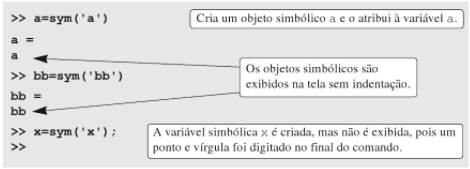
\includegraphics[scale=1]{Figuras/objeto_simbolico.png}
  \caption{Criação de objeto simbólico no Matlab \cite{2012:Amos}}
  \label{objeto_simbolico}
\end{figure}

O Matlab trabalha com os conteúdos da Álgebra Linear para a resolução de problemas, assim através do mesmo é possível encontrar a solução de sistemas de equações lineares, por exemplo, considerando o exemplo (I), a entrada e resolução no Matlab seria de acordo com o código a seguir:

\begin{center}
(I)
    $\left\{\begin{matrix}
        x_{1} + 2x_{2} + x_{3} = 8 \\ 
        2x_{1} - x_{2} + x_{3} = 3 \\ 
        -x_{1} + x_{2} - 2x_{3} = -5  
    \end{matrix}\right.$
    \label{equacao}
\end{center}

Código Matlab, resolução sistemas de equações lineares:

\begin{lstlisting}
    A=[1 2 1; 2 -1 1; -1 1 -2]
    A =
        1   2   1
        2   -1  1
        -1  1   -2
    b=[8;3;-5]
    b =
        8
        3
        -5
    x = inv(A)*b ou x = A\b ou x = pinv(A)*b
    //Mostrando o resultado
    x =
        1
        2
        3
\end{lstlisting}

Essa resolução não está em nível de computação simbólica, mas para resolução, basta somente utilizar o comando $sym$ para criar um objeto, como descrito na figura \ref{objeto_simbolico} e desenvolver a questão.


\section{Metodologia de Desenvolvimento Ágil}
\noindent Um ponto importante das metodologias ágeis é que elas são adaptativas, ou seja, elas podem ser adaptadas no decorrer do desenvolvimento de \textit{software} a novos fatores, o que é diferente das metodologias clássicas, a qual pode acontecer de no decorrer do desenvolvimento de um \textit{software} realizar todas as etapas necessárias para sua concretização e depois verificar que elas não atendem mais ao propósito que foi implementado. Isso porque as regras podem ter mudado e para a realização das adaptações pode ter um custo alto, desse modo, não sendo proveitoso desenvolvê-las. Foi a partir dessa situação que a crise do \textit{software} começou a crescer, visto que os \textit{software} não satisfaziam os clientes ou empresas \cite{2005:rezende}.

\subsection{Manifesto Ágil}
\noindent O manifesto ágil teve seu surgimento em 2001 pelo engenheiro de \textit{software} Kenet Beck\footnote[5]{Kenet Beck é um engenheiro de \textit{software}, responsável por criar o \textit{Extreme Programming e Test Driven Development (TDD)}} e mais 16 (dezesseis) desenvolvedores de sistemas de grande destaques na área, a qual batizaram de \textit{``Agile Alliance"} e assinaram um documento conhecido com \textit{``Manifesto para Desenvolvimento Ágil de \textit{Software}"} como registro dessa prática de desenvolvimento \cite{2001:Pressman}.

Atualmente o processo de desenvolvimento de \textit{software} utilizando a metodologia ágil tem ganhado bastante espaços devido ao fato que Pereira \cite{2013:Pereira} relata:
\begin{quote}
    os processos ágeis de desenvolvimento compartilham a premissa de que o cliente aprende sobre as suas necessidades, na medida em que é capaz de manipular o sistema que está sendo produzido e, com base no \textit{feedback} do sistema, ele reavalia as suas necessidades e prioridades, criando mudanças que devem ser incorporadas ao \textit{software} (\cite{2013:Pereira}, apud \cite{2004:Teles}, 2004). 
\end{quote}

\subsection{\textit{Framework Scrum}}
\noindent Dentre as metodologias ágeis atualmente presentes no mercado, existe o \textit{ framework Scrum}, esta criada em 1990 por Jeff Sutherland e sua equipe de desenvolvimento, mas somente na década seguinte que se tornou popular. Recentemente Scwaber Beedle foi o responsável por adicionar novas atualizações na metodologia \cite{2001:Pressman}. Tal ferramenta aborda todos os princípios utilizados pelo o manifesto ágil, visando a orientação sobre o desenvolvimento de \textit{software} nas atividades de requisitos como levantamento e análise de requisitos, planejamento do projeto, evolução e entrega do produto são atendidos.

O \textit{Scrum} funciona de acordo com seu ciclo de atividades como a figura \ref{chave_para_refencia_cruzada} é demonstrada.

\begin{figure}[!hb]
  \centering 
  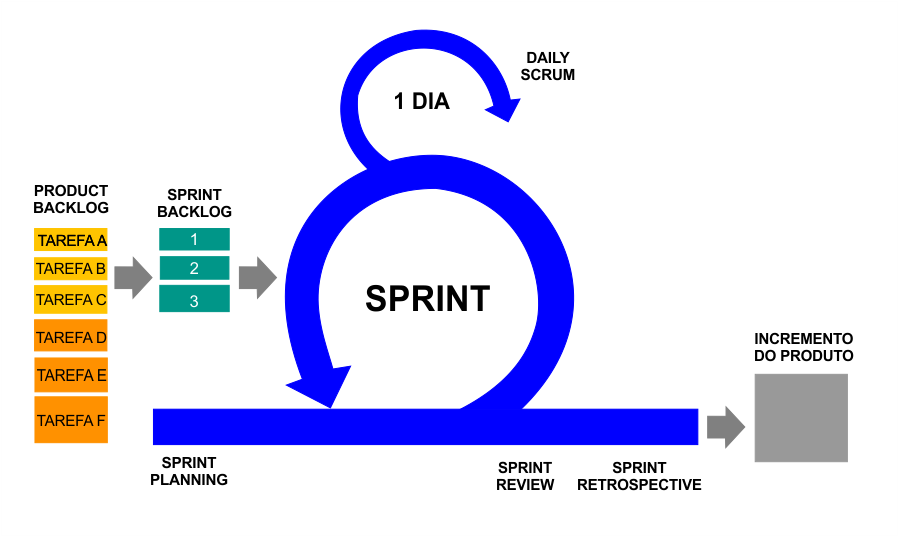
\includegraphics[scale=1.8]{Figuras/ciclo_scrum.png}
  \caption{Ciclo de atividades da metodologia \textit{Scrum}. Adaptado de \cite{0000:rafael}}
  \label{chave_para_refencia_cruzada}
\end{figure}

No decorrer do desenvolvimento vários termos são utilizados para descrever cada etapa, tais como \textit{Product Backlog, Sprint Backlog, Daily Scrum Meeting, Sprint Review Meeting,} entre outras. Adiante serão expostas cada uma com sua importância e significado dentro da metodologia.

\subsubsection{\textit{Product Backlog}}
\noindent O \textit{Product Backlog} consiste em uma lista que nela estarão elencadas tudo que acredita que será produzida ao longo do projeto e os itens presentes nela serão desenvolvidas pelo \textit{Scrum Team}, ou seja, a equipe de desenvolvimento e essa é a única fonte de trabalho que a equipe realiza. E é nela que irão conter todas a necessidades e objetivos de negócio do cliente e as partes interessadas do projeto \cite{0000:rafael}. Essa lista é categorizada com níveis de prioridades e essas prioridades são estabelecidas pelo \textit{Product Owner}.

A figura \ref{chave_para_refencia_cruzada} demonstra como é estruturada a lista de \textit{Product Backlog}, sendo organizada por prioridades. 

\begin{figure}[!htb]
  \centering 
  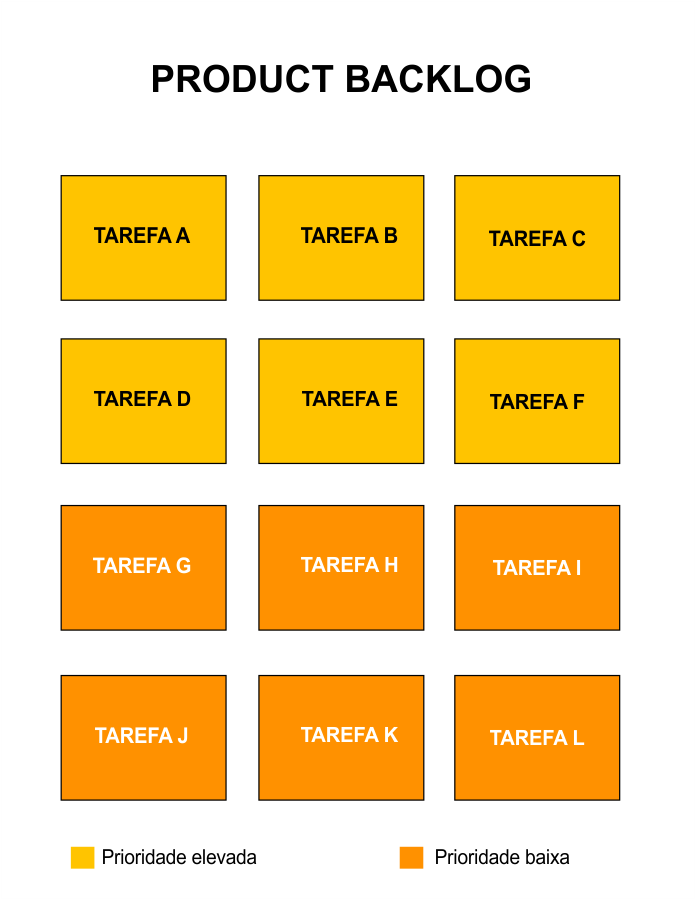
\includegraphics[scale=1.2]{Figuras/product_backlogs.png}
  \caption{Estrutura de um \textit{Product Backlog}. Adaptado de \cite{0000:rafael}}
  \label{chave_para_refencia_cruzada}
\end{figure}

\subsubsection{\textit{Sprint Backlog}}
\noindent Uma \textit{Sprint} de acordo com Kotonya \cite{1997:Kotonya} consiste em um planejamento que visa avaliar a situação do trabalho, os recursos alocados para o desenvolvimento são selecionados e o \textit{software} é implementado. Desse modo, ela é basicamente uma lista que o time de desenvolvimento se compromete a realizar as tarefas presentes. Uma \textit{Sprint} é criada no primeiro evento realizado no ciclo, que é a \textit{Sprint Planning}. Durante a \textit{Sprint} a equipe de desenvolvimento verifica o quadro e solicita a tarefa que acredita que irá conseguir desenvolver e levando em consideração as prioridades de cada.

A figura \ref{chave_para_refencia_cruzada} demonstra a estruturação de um quadro de \textit{Sprint}, sendo que é dividido em tarefas que tem para fazer, as que estão em desenvolvimento e as que já estão feitas.

\begin{figure}[!htb]
  \centering 
  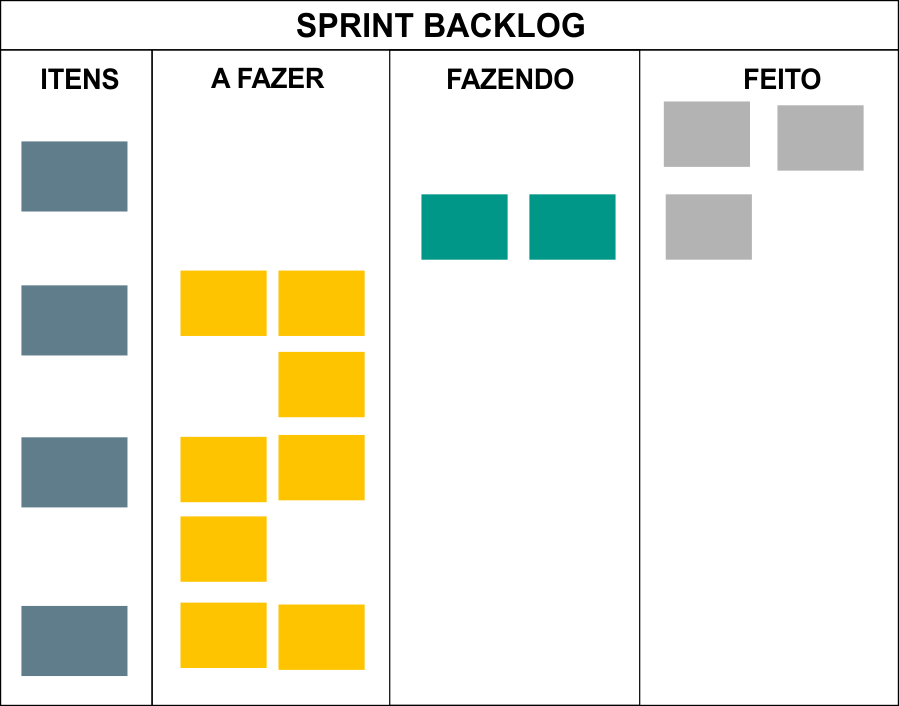
\includegraphics[scale=1.5]{Figuras/sprint_backlog.png}
  \caption{Quadro de tarefas de uma \textit{Sprint Backlog}. Adaptado de \cite{0000:rafael}}
  \label{chave_para_refencia_cruzada}
\end{figure}

\subsubsection{\textit{Daily Scrum Meeting}}
\noindent Todos os dias que os \textit{Sprints} são realizadas a equipe de desenvolvedores, \textit{Product  Owner},\textit{Scrum Master} e outras pessoas, sendo que estas só poderão escutar, participarão de uma reunião que apresenta como objetivo disseminar conhecimentos sobre o que foi realizado no dia anterior e assim conseguir identificar problemas que estão atrapalhando o desenvolvimento e nela são priorizados o trabalho que será realizado no dia.

\subsubsection{\textit{Sprint Review Meeting}}
\noindent Assim como antes de iniciar um \textit{Sprint} é realizado uma reunião para disseminação das informações, no final de cada \textit{Sprint} é realizado também uma reunião que essa apresenta como objetivo de demonstrar o que foi desenvolvido durante o dia, a qual nela participarão toda a equipe, como o \textit{Product Owner, Scrum Team, Scrum Master}, gerência, clientes e engenheiros.

\subsubsection{\textit{Product Owner}}
\noindent Esse é um dos principais personagens da metodologia \textit{Scrum}, pois ele é o responsável por garantir e maximizar o trabalho da equipe, sendo ele que define os itens que irão compor o \textit{Product Baclog}. A partir do momento em que a equipe compromete-se em desenvolver as atividades no \textit{Sprint} ele se compromete a não trazer novos requisitos para \textit{Scrum Team}.

\subsubsection{\textit{Scrum Master}}
\noindent O \textit{Scrum Master} apresenta como função dentro da metodologia de assegurar que a equipe respeite e siga os valores e práticas do \textit{Scrum}, bem como também é o responsável por resolver qualquer impedimento que venha surgir no decorrer da \textit{Sprint}.

\section{Avaliação da aprendizagem}
\noindent A prática de avaliar o aprendizado está presente em todos os momentos da vida acadêmica de um estudante, visto que essa prática faz parte dos objetivos das escolas. E a avaliação de acordo Libâneo \cite{1990:libaneo} não se restringe somente ao processo de realizar provas e atribuir notas, ela é bem mais complexa, pois tem o papel de cumprir as funções pedagógicas-didáticas que se refere ao papel da avaliação seguindo os objetivos gerais e específicos da educação escola, de diagnóstico e de controle em relação aos níveis de rendimento escolar. E esta é uma tarefa necessária e permeante do trabalho do docente. Desse modo, o autor a define como sendo uma reflexão sobre as condições de qualidade do trabalho dos dois personagens principais da academia, os professores e os alunos.

Silva \cite{2015:Silva} apresenta um conceito sobre avaliar parecido com o de Libâneo \cite{1990:libaneo} em que a avaliação não restringe somente no processo de atribuir notas ou conceito para os discentes, mas sim conseguir identificar os espaços que são deixados no decorrer do aprendizado e assim analisar e aplicar estratégias a fim suprir as necessidades identificadas.

Para Datrino \cite{2010:Datrino} na definição de avaliação existem alguns itens que são considerados elementos chaves, sendo eles: julgamento, apreciação, valoração e qualquer efeito que implicar em julgar. Apesar de avaliar implicar medição, a avaliação é algo que é bem mais abrangente do que simplesmente realizar a medição ou qualificação de alguém para saber se adquiriu os conhecimentos.
